% v2-acmtog-sample.tex, dated March 7 2012
% This is a sample file for ACM Transactions on Graphics
%
% Compilation using 'acmtog.cls' - version 1.2 (March 2012), Aptara Inc.
% (c) 2010 Association for Computing Machinery (ACM)
%
% Questions/Suggestions/Feedback should be addressed to => "acmtexsupport@aptaracorp.com".
% Users can also go through the FAQs available on the journal's submission webpage.
%
% Steps to compile: latex, bibtex, latex latex
%
% For tracking purposes => this is v1.2 - March 2012
\documentclass{acmtog} % V1.2
\usepackage{comment}
\usepackage[utf8]{inputenc}
\usepackage[swedish,english]{babel}
\usepackage[T1]{fontenc}
\usepackage{natbib}
\usepackage{epigraph}
\usepackage{csquotes}
\usepackage{url}
\usepackage{graphicx}
\usepackage{tabularx}

% CUSTOM SETTINGS
\setlength{\epigraphwidth}{.3\textwidth}

%%%%%%%%%% DOCUMENT %%%%%%%%%%
\begin{document}

\markboth{Carl-Johan Backman}{Discovering Data-Driven Stories: A Case Study}

%\title{Spreading a Fact-Based Worldview\\ \large{Narrative Information Visualization Through User-Centered Data Stories}} % title

\title{Discovering Data-Driven Stories: A Case Study \\
Läsardrivna narrativ i datavisualiseringar: En fallstudie
}

\author{Carl-Johan Backman
\affil{KTH Royal Institute of Technology}
\affil{Gapminder Foundation}
}
\maketitle

\begin{abstract}
Narrative visualization is a young and emerging field, driven mainly by data journalists. For this reason, most data stories available today are author-driven. However, with the rise of interactive visualizations the possibilities for creating reader-driven stories have become apparent. 

In this thesis, we present a straigthforward prototype, AsylKoll, built to support the articulation of reader-driven stories about Swedish immigration during 2015. We test its ability to support reader-driven stories by performing two user-studies based on the Think Aloud Method. In particular, we evaluate the prototype along the dimensions of reader engagement and learning. We find that user-centric data and various effects, such as transitions and mouse-overs, have a positive impact on reader engagement. In addition, we find that typical tasks such as extracting extremes and making comparisons are very important for users to gain insight and learn from the data. Foremost, this thesis shows the potential that simple, interactive visualizations have to make people engage and gain insights from data.
\keywords{Narrative visualization, data visualization, think aloud method.} 
\end{abstract}

\begin{abstract}
Att skapa faktabaserade narrativ med hjälp av datavisualiseringar är någonting som blir allt mer vanligt idag. Utvecklingen drivs framför allt av datajournalister och av den anledningen är det typiskt sett författar-drivna historier som berättas. På senare tid har det dock blivit allt lättare att utveckla avancerade, interaktiva visualinsergar och det har öppnat för skapa faktabaserade narrativ drivna av läsaren istället. 

Läsar-drivna narrativ är det som vi utforskar i den här studien. Med hjälp av en prototyp som vi byggt, AsylKoll, som visar statistik från asylinvandringen till Sverige under 2015, undersöker vi vad som krävs av en visualisering för att användare ska kunna härleda sina egna faktabaserade historier från den. Vi kollar i synnerhet på hur man kan uppmana användaren att interagera med verktyget samt vad som krävs för att användaren ska lära sig från datan. 

Verktyget testas genom två användarstudier med 'Think Aloud'-metoden. I studien  finner vi att data centrerad kring användaren och olika typer av effekter, såsom transitioner och mouse-overs, påverkar användarens vilja att interagera med visualiseringarna positivt. Vidare finner vi även att typiska funktioner som exempelvis möjligheten att snabbt hitta extremvärden samt att kunna göra olika jämförelser av data, är viktigt för lärandet. 
\end{abstract}

\section{Introduction}
\label{sec:intro}
\begin{comment}
Something about fact-based worldview

Somthing about refugee crisis in Europa....focus on Sweden. A large debate, a lot of numbers thrown around. Do people know how many refugees there municipality has accepted?

Understanding how people find stories is a way to understand how discover facts. Finding a story in a dataset, using interactive visualization where you can filter, brush etc, is nothing else than making sense of the data. A quest for understanding.

Want a tool that is not too complicated to use. Not too complicated visual mappings. Simply charts which provides support for simple features such as filtering, zooming.


* Viktigaste frågan bland svenska folket
* Stora förändringar (skärpt asylpolitik)
* Heta känslor, starka åsikter, kraftig polarisering öppnar upp för rykten, lögner och annan missvisande information. Med väldigt stora konsekvenser

\end{comment}

Prior to any proper decision, big or small, we need information. In particular, we need fact-based information, to gain an understanding of the world to which the consequences of the decision applies. However, while we have information in abundance today, it is often hard to tell the fact-based information from the deceptive noise. There is a subtle difference between data-driven and data-manipulated stories that has to do with intent and transparency. Given access to raw data is transparent and the only explicit intent is empowerment of individuals.

In Sweden, one topic where this difficulty is apparent, is the public debate regarding the refugee situation. It has been a widely and increasingly debated topic in recent years \cite{dn}. During the ongoing refugee crisis in Europe, Sweden is one the of countries which has taken the greatest responsibility in offering people fleeing from war and terror a safe place to stay. In fact, Sweden received more refugees per capita in 2015 than any other European country. During the same year, more than 160 000 refugees applied for asylum in Sweden, comparable to almost 2\% of the total Swedish population \cite{migrationsverket}. However, the situation has also generated a heated debate and a polarized population. Those who are in favor of welcoming more refugees versus those who want to close the borders. As a consequence of this heated debate, misleading information stemming from doubtful sources frequently arise on social media and alternative media.

In this thesis, we aim to create and test a transparency tool that puts in the hands of individuals, interactive and visual access to the raw data regarding refugee migration towards Sweden in 2015. We report the design process and the results from pilot studies with seven Swedish citizens.

\subsection{Background}
\label{sub:background}
The decisions made by elected politicians in Sweden are inevitably shaped by the public opinion. Moreover, the decisions made regarding this specific issue, immigration, affect the fates of families fleeing from war. Hence, the importance and severity of the debate to be carried out with correct facts and figures cannot be underestimated. Therefore, the first step when participating in such a debate should be to obtain a fact-based view of the current situation. Luckily the data about the refugee situation in Sweden is not difficult to obtain. It is publicly available on the Swedish Migration Agency's web page \cite{migrationsverket}. However, the data is published in table format through excel sheets and PDFs and, because of that, hard for the general public to analyze and process.

For this reason, we have created AsylKoll\footnote{https://people.kth.se/\textasciitilde cjba/thesis/} (Vizylum in English), a tool for exploring the datasets published by The Swedish Migration Agency. It is a web-based tool built on HTML, CSS and Javascript. The focus has been to create a tool easy to access and use for non-experts. The tool will be described in greater detail in Section \ref{sec:tool}.

\subsection{Motivation}
\label{sub:motivation}
The work presented in this thesis is motivated by the increasing interest and use of information visualization to convey stories about data. This growing interest and practice of narrative visualization is most notable among journalists but lately also in the scientific world \cite{eccles2008stories,ma2012scientific}. While research in information visualization, historically, has focused on data analysis and exploration there has been a slight shift in recent years \cite{kosara2013storytelling}. Presentation and communication have attracted more attention and research about narrative visualizations is becoming more established. Despite that, there is a lack of studies that evaluate if the actual effects stories have on a reader are the same as those the author intended. Most of the current research focuses instead on how the visualizations are designed and framed. Another insufficiently research subject is that of \emph{reader-driven stories}, as defined by \cite{segel2010narrative}. Most narrative visualizations constructed today are made by journalists who have already decided on a story to tell. In that sense, narrative visualizations are currently \emph{author-driven}, to a large extent. 

However, in this age of information the amount of data in our societies is continuously increasing and while the data can be relevant to the public, only a fraction will be analyzed and presented as stories by journalists. For that reason we believe that reader-driven stories can play an important role in spreading a fact-based world view. By providing tools for the general public, which can then be used to explore data relevant to them and let them find stories of their own.

Yet another important motivation behind this study is its use for \emph{Gapminder Foundation}, where this thesis was conducted \cite{gapminder}. Gapminder is currently developing a framework for building visualization tools, called \emph{Vizabi} \cite{vizabi}. Gapminder strives for spreading a fact-based world view and tries to achieve this by making data on global development easily accessible to the general public. It wants people to explore the data by themselves, using tools such as Vizabi, and by that gain a better understanding of the world. In other words, Gapminder wants readers to derive their own stories from the data that the foundation gathers. Hence, the insights drawn from this thesis will be valuable in the continuing development of Vizabi.

Taking all the above into account, AsylKoll was constructed as a narrative visualization intended to support the articulation of reader-driven stories, by non-experts. We have evaluated the tool through user-studies in focus groups. In particular, we wanted to explore reader-driven stories along the dimensions of reader engagement and learning.

Since reader engagement and learning, or memorability, are desired outcomes of many narrative visualizations this research should be valuable to a large fraction of the community involved with creating such narratives. Especially journalists and educators ought to benefit from this work, since they often share a similar desire to catch the readers' interest, encourage the readers to explore the data by themselves and still learn the story intended by the author. 

To summarize, our two primary contributions with this research are:
\begin{itemize}
\item Provide a tool for non-experts to access, explore and gain knowledge from The Swedish Migration Agency's public refugee data in Sweden
\item Provide insights about reader-driven stories, narrated by non-experts, especially along the dimensions of \emph{reader engagement} and \emph{learning}
\end{itemize}

\subsection{Research Question}
\label{sub:rq}
As described above, in this thesis we set out with a desire to learn more about reader-driven stories and if AsylKoll can be used as tool for facilitating them. More specifically, we try answer the question: 

\begin{displayquote}
How well does AsylKoll support the articulation of reader-driven stories, for non-experts, grounded on geographic-centric data?
\end{displayquote}
The term \emph{non-experts} is a loosely defined term used in this thesis to describe the general public, which has no particular experience or knowledge about data analysis, statistics and data visualization. Moreover, we target the Swedish population and therefore, the language in the user interface is Swedish. 

By trying to answer the question posed above, we also hope to gain further insights about reader-driven stories and what non-experts need for deriving data-driven stories of their own.

% TODO: Something about the method, and results

\subsection{Outline}
\label{sub:outline}
This thesis is structured as follows. In the next section, Section \ref{sec:relwork}, we will list and present the most relevant work done in the area of narrative visualization. Then, the tool is presented in greater detail, including the data which it visualizes, in Section \ref{sec:tool}. Following this, in Section \ref{sec:method}, we will describe the method used to evaluate AsylKoll. In Section \ref{sec:results}, we present the results of our user-studies. Subsequently, the results are analyzed and discussed in Section \ref{sec:discussion}. Lastly, the thesis is summarized along with our conclusions and reflections on future work in Section \ref{sec:conclusion}.

\section{Related Work}
\label{sec:relwork}
%\epigraph{\scriptsize [That is] the essential dilemma of narrative designs - how to reduce the magnificent four-dimensional reality of time and three-space into little marks of paper flatlands.}{\scriptsize Envisioning Information (1990)\\ Edward Tufte}

Below we list and discuss previous work conducted in the same research area as this thesis and how they relate. We start by defining the scope of narrative visualization.

\subsection{Narrative Visualization}
\label{sub:narr_vis}
Narrative visualization is a young and emerging field within information visualization. Due to this, the subject \emph{narrative visualization} has been loosely defined so far, and still is. \citet{lee2015more} tries to give one definition of visual data stories as something that fulfills all of the following three conditions: i) a story that consists of story pieces backed up by data; ii) most of these pieces are visualized to support one or more intended messages; and iii) the pieces are presented in a meaningful order or with some connection between them to support the author's high-level communication goal. Thus, we can say that this definition emphasizes the importance of data, visualizations the and presentation of them. We adhere to the definition of \citet{lee2015more} in this thesis, however, since we are focusing on reader-driven stories, \emph{the author} and \emph{the intended messages} will in most cases mean the readers and their intended messages. The only high-level communication goal that we, as authors have, is to spread a fact-based world view. In particular, to spread a fact-based view of the asylum status in Sweden, during 2015.

Looking back in time, one of the first to acknowledge the potential of storytelling in information visualization were \citet{gershon2001storytelling}. In the paper they present a number of methods that can be used to build a story effectively using visualizations, which in their case is a story about a hostage situation. Even though the authors do not actually describe any data visualizations in detail, they argue that storytelling is a particularly useful tool for conveying key information to the reader. In the same way, we believe that discovering those stories on your own can be a powerful method for readers to grasp and understand facts about the world.

Comparing to classical information visualization there is an important distinction between it and narrative visualization. The former tends to focus on analysis and the ability to explore the datasets which it maps, while the latter is more focused on the presentation and communication of insights concealed in the data. The implications of this has been that information visualization in general have focused on experts (e.g. statisticians, scientists), who might be used to working with data and need tools to explore it accurately. Narrative visualization is different, since it often targets non-expert readers that are not used to data analysis or statistics. Indeed, this is the audience we target in this study. This shift in target groups has important implications when constructing the stories. One important implication, recognized in several studies, being that of the text accompanying the visualizations \cite{borkin2016beyond,segel2010narrative}.

In their paper, \citet{segel2010narrative} review the design space of narrative visualization and classify different genres. The authors identify seven genres and give some general advice on how one can design narrative visualizations. In addition, they reflect on ways of balancing \emph{author-driven} versus \emph{reader-driven} stories. \citet{segel2010narrative} note that while storytelling, historically, have had more of an author-driven structure, new information visualizations open up for interactivity and reader-driver stories. This is the area of research that we explore in this thesis.

The design space is, however, only one side of narrative visualization. Another equally important aspect is what effect the stories have on the readers. This is touched upon by \citet{hullman2011visualization}, when they investigate how different rhetorical decisions regarding how to frame a story, something the authors call \emph{visualization rhetoric}, affect readers' interpretations of the story. This research has been extended by \citet{hullman2013deeper} into showing how to effectively sequence the visualizations in a story. They find that it is most effective to sequence by a temporal ordering and worse to sequence on granularity. Conclusions that we draw on when designing AsylKoll.

\subsection{Reader Engagement}
\label{sub:reader_engagement}
With the interactive information visualizations available today a common goal of designers is to create visualizations that encourage the reader to engage with the data and explore it. Something that is particularly essential if we want to create a tool which facilitates reader-driven stories. One example of increasing reader engagement is given in \citet{diakopoulos2011playable}, where the author tries to accomplish this through the usage of game mechanics. This approach has some interesting implications. By constructing the story as a game, the story is governed by the structure of the game, however, not bound by a linear sequencing as stories usually are. The game structure of the stories is found to increase the reader engagement, while decreasing the potential for insights and learning.

Another suggestion to increase reader engagement can be found in \citet{yousuf2014constructing}. The authors present their framework, VisEN, which dynamically creates personalized narratives as the reader explores the data. They find that these automatically generated and personalized stories have a positive impact on the reader's learning by increasing and improving their engagement with the data. Related to this research, albeit not exactly the same, is that of \citet{boy2015can}. Contrary to \citet{yousuf2014constructing}, they find that the use of stories in relation to interactive visualizations do not increase the reader engagement. 

\citet{moere2011role} argue for the importance of aesthetics when designing information visualizations. The authors mean that a \emph{''highly aesthetic representation may compel the user to engage with the data''}. To assist in this work they provide a model of design in information visualization. The model defines three design domains - visualization practice, visualization studies and visualization exploration - which all have specific implications for design considerations. Moreover, aesthetics is an important factor to take into account when trying to create memorable visualizations.

All in all, it is safe to say that current research cannot really give a good answer on how to increase reader engagement. While the research described above in general focuses on the presentation of data and the design of the visualizations, we will in this thesis instead try to increase reader engagement by focusing on the data, i.e. by choosing geographic-centric data made relevant to the user. 

\subsection{Learning}
\label{sub:learning}
Constructing stories that the reader learns from and remembers, is of interest for anyone trying to convey a message. There is an ongoing debate in the research society on how to design memorable visualizations. For a long time the consensus in information visualization was to keep the charts and visualizations as plain and minimalistic as possible. Implying that decorative and other non-related imagery, also called ''chart junk'', ought to be be avoided \cite{tufte1983visual}. \citet{bateman2010useful} go against this consensus and argue that chart junk does not affect readers interpretation accuracy but it does, however, increase the recall of the visualizations. 

\citet{borkin2013makes} and \citet{borkin2016beyond} draw similar conclusions when investigating what makes visualizations memorable. They find that very plain charts and visualizations (compared to more uniquely designed) are difficult for readers to remember. In addition, they find strong evidence for the importance of using titles and annotations to make the story memorable. However, the authors also acknowledge the difficulty in ensuring that the readers remember the \emph{right} thing: \emph{''We do not want just any part of the visualization to stick (e.g. chart junk), but rather we want the most important and relevant aspects of the data or trend the author is trying to convey to stick.''} \cite{borkin2013makes}.

We will take a more conservative stand with regards to chart junk in this thesis, i.e. avoiding it and instead sticking to rather minimalistic charts, for reasons that will be explained in greater detail in \ref{sec:tool}. We are, however, guided by the research underlining the importance of the text accompanying the visualizations, especially the titles.

\section{AsylKoll}
\label{sec:tool}
In this section we present our tool, \emph{AsylKoll}. A tool for exploring the datasets published, on a monthly basis, by The Swedish Migration Agency. AsylKoll is built targeting non-experts and the implications of this decision will be discussed later in this section. Moreover, as often is the case when designing information visualizations, a guiding mantra through the designing process has been that given by \citet{shneiderman1996eyes} \emph{''overview first, zoom and filter, then details-on-demand''}. However, before we get into the details of the visual mappings and the motivation behind them, in Section \ref{sub:visuals}, we start by briefly presenting the data shown in the tool.

\subsection{The Data}
\label{sub:data}
All the data which is visualized or presented in some way, through AsylKoll, comes from three providers: The Swedish Migration Agency, Statistics Sweden (SCB) and Ipsos \cite{migrationsverket,scb,ipsos}. 

As explained in the introduction we chose to work with immigration data since it is such a heavily debated subject and rated as the most important political topic by Swedes in 2015 \cite{svt,dn}. We also decided to include population data from SCB to use in conjunction with the immigration data, to enable comparisons and put the immigration data in a local context. In addition, we incorporated some poll data on the public opinion regarding refugees, since we believed that adding Swedes perceptions on this subject would help give a better overview of the refugee status in Sweden.

All the data was cleaned and preprocessed using Python Pandas \cite{pandas}.

\subsection{The Visuals}
\label{sub:visuals}
\subsubsection{Technical Details}
AsylKoll\footnote{https://people.kth.se/~cjba/thesis/} is built on HTML, CSS and Javascript (jQuery, D3.js), with D3.js constituting the core of the visualizations \cite{d3}. The motivation behind making AsylKoll a web application is accessibility. Since the essential goal is to spread a fact-based world view, those facts should be distributed to an as large share of the population as possible. Also, it is well aligned with Gapminder's vision to be \emph{''a modern 'museum' that helps making the world understandable, using the Internet''} \cite{gapminder}.

D3.js is well suited for web visualization, since it is a powerful library for manipulating DOM documents which, in addition, is supported natively by most modern browsers. Some visualizations in the tool are built directly using D3 while others, simpler visualizations, such as bar charts and columns charts, are created using C3.js \cite{c3}. C3 is a visualization framework built on top of D3.js. The reason for using C3.js is its default support for filtering and details-on-demand, while being customizable and easy to set up and use.

Furthermore, accessibility is enhanced by the complete responsiveness of the site. All the charts, including the web page itself is responsive.

\subsubsection{General Ideas}
\label{subsub:general_ideas}
As an attempt to minimize the time spent on figuring out how the visualizations work and what they show, we have tried to limit the complexity of the visual mappings by using well-known types of charts. Such as maps, bar charts and column charts. This is a decision which most likely will decrease the memorability of the charts themselves, but as AsylKoll is a tool for the users to discover stories by themselves, we believe that an innovative design might accidentally take attention away from this task. Especially since it is hard to ensure that users remember the \emph{right} thing \cite{borkin2013makes}.

To further assist the user we have drawn on previous research and spent time on trying to use descriptive titles and keeping the explanatory text as precise and short as possible \cite{borkin2016beyond,borkin2013makes,segel2010narrative}.

Learning from \citet{hullman2011visualization} and \citet{hullman2013deeper}, we have used temporal ordering as often as possible, to ease the cognitive processing of the data.

AsylKoll consists of two main views - \emph{the arrivals view} and \emph{the asylum view}. These are described one by one below. Also, as mentioned earlier in this section, the design process has been guided by the visualization mantra \emph{''overview first, zoom and filter, then details-on-demand''} and as we describe the views we will do so along the tasks discussed in \citet{shneiderman1996eyes}, namely: overview, zoom, filter, detail-on-demand, relate, history and extract. Note, however, that AsylKoll is in an early stage of the development phase and thus, the tool does not support all of these tasks. 

\subsubsection{The Arrivals View}
\label{subsub:view1}
The arrivals view shows data on asylum seekers who have been granted asylum and have been placed in some Swedish municipality. This group of asylum seekers is called \emph{arrivals} in this thesis. The arrivals can end up in a municipality for five different reasons, defined by The Swedish Migration Agency. The reasons are briefly described below.

\begin{enumerate}
\item \textbf{Quota Refugee} - a refugee that has been elected abroad through a collaboration between The Swedish Migration Agency and the UN.
\item \textbf{Arranged Accommodation} - asylum seeker who has been granted resident permit and then been placed in a municipality by The Swedish Migration Agency or The Swedish Labor Agency.
\item \textbf{Self-Arranged Accommodation} - asylum seeker who has been granted resident permit and who has arranged with accommodation by himself or herself.
\item \textbf{Secondary Immigration} - a family member to an asylum seeker who has been granted resident permit and is already living in some municipality in Sweden.
\item \textbf{Miscellaneous} - mainly individuals who have been granted resident permit without applying for asylum. 
\end{enumerate} 

The starting frame of the arrivals view shows an overview of where all the arrivals have ended up in Sweden, both in actual numbers and per capita (see Figure \ref{fig:view1_start}). To support the understanding of this data the tool makes use of a map of Sweden, next to a bar chart. The map is a choropleth, where the counties are colored by number of arrivals per capita. The bar chart accompanying the map shows the number of arrivals per county, in actual numbers. This initial frame provides an \emph{overview} of the numbers of arrivals in Sweden during 2015 and the two graphs together enable the users to \emph{relate} per capita numbers to absolute numbers.

\begin{figure*}
\centering
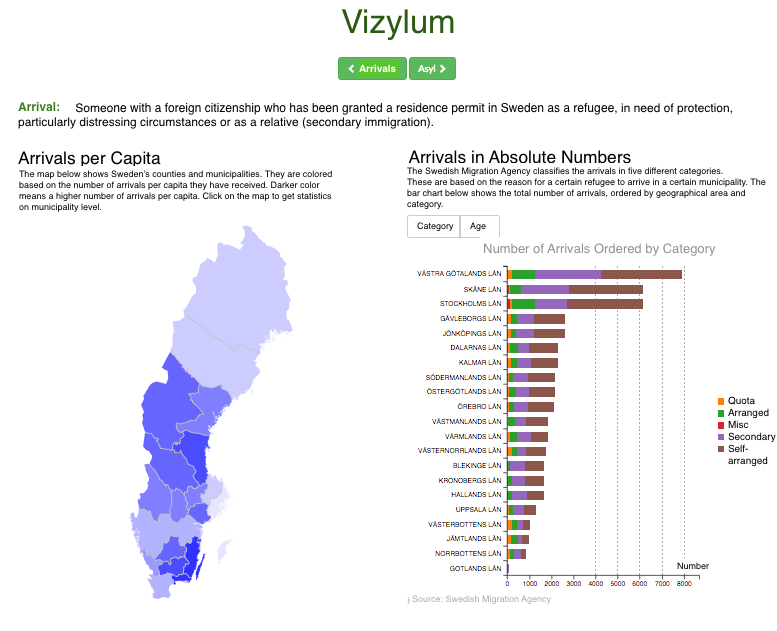
\includegraphics[width=\textwidth]{img/view1_start_en.png}
\caption{Starting frame of the arrivals view. Showing a choropleth map, colored by arrivals per capita, and a bar chart showing the number of arrivals in absolute numbers. Note: the text has been translated to English in this thesis, however, the web app is in Swedish. For a short video showing the tool, follow this link: https://vimeo.com/187571807.}
\label{fig:view1_start}
\end{figure*}

The bar chart is a stacked bar chart with two options for grouping. One where the data is grouped by reasons for arrival (see list above) and one where the arrivals are grouped by age. Also, it is possible to \emph{filter} the data in the bar chart by hovering and clicking the legend.

Moreover, the view provides a drill down feature, down to municipality level, by clicking on a specific county. Hence, it is possible to \emph{zoom} and \emph{filter} the data by county. When drilling down the map itself will zoom in on the county and color municipalities based on arrivals per capita instead (see Figure \ref{fig:view1_zoom}). The rest of the counties are colored gray in order not to steal focus from the selected county. The bar chart will also update. It shows the same data as earlier but per municipality instead, in the selected county. 

\begin{figure*}
\centering
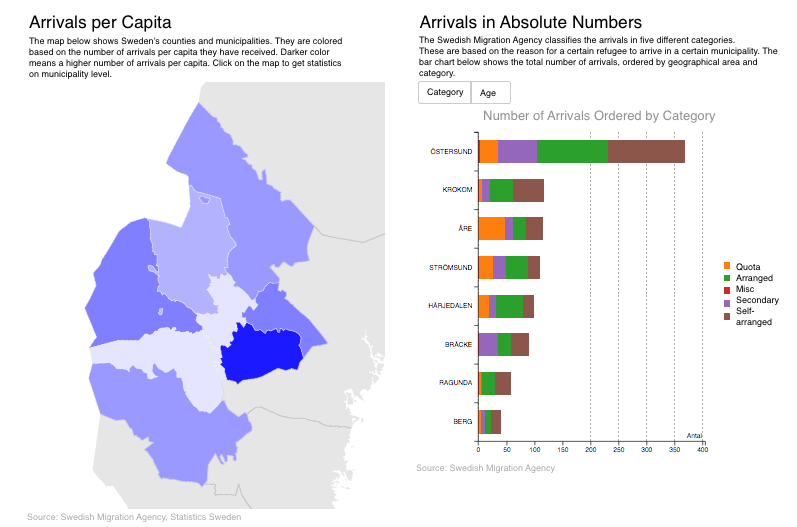
\includegraphics[width=\textwidth]{img/view1_zoom_en.png}
\caption{The arrivals view when zoomed in on a particular county. The municipalities within the selected county is colored by arrivals per capita. The bar chart is also updated, showing data on municipality level instead. Note: the text has been translated to English in this thesis, however, the web app is in Swedish. For a short video showing the tool, follow this link: https://vimeo.com/187571807.}
\label{fig:view1_zoom}
\end{figure*}

In the zoomed in view, another column chart will appear too, which shows the arrivals by country of origin, in the selected county (see Figure \ref{fig:view1_citizenship}). This will give a better \emph{overview} of who has moved to that particular county and also humanize the arrivals data.

Finally, the map and the bar chart both give the user \emph{details-on-demand} on mouse-over, in the zoomed in view as well as the zoomed out view.

\begin{figure*}
\centering
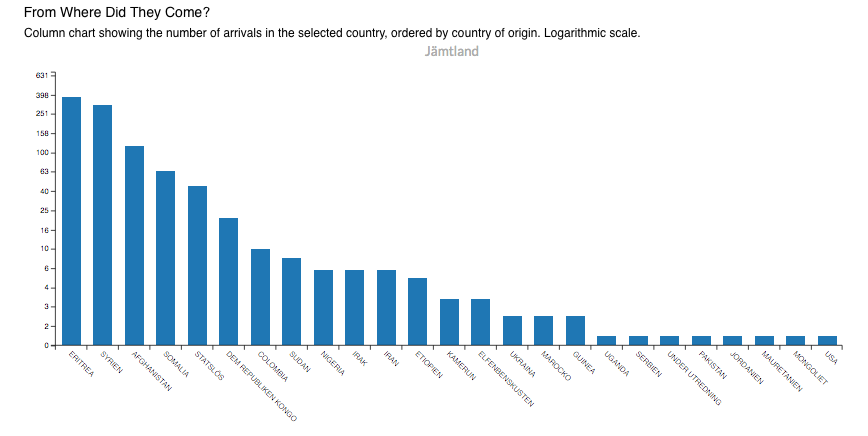
\includegraphics[width=\textwidth]{img/view1_citizenship_en.png}
\caption{The column chart that appears when zooming in on a county. The chart shows the number of arrivals per country of origin, sorted in descending order. Note: the text has been translated to English in this thesis, however, the web app is in Swedish. For a short video showing the tool, follow this link: https://vimeo.com/187571807.}
\label{fig:view1_citizenship}
\end{figure*}

\subsubsection{The Asylum View}
\label{subsub:view2}
The other main view, the asylum view (see Figure \ref{fig:view2}), is made up of two charts and some key facts expressed in plain text. The main chart is a combination chart consisting of a column chart and a line chart. The columns express the number of asylum applications, the number of decision made in asylum cases (on whether or not to grant asylum) and the number of people who was granted asylum. The data is presented by month, to show the \emph{history} of the asylum immigration over the year. The line chart which accompanies the column chart shows the average handling time per case, in days. Together this combination chart gives a thorough \emph{overview} of the status of the asylum immigration in Sweden during 2015. It provides insights about when most asylum seekers arrived to Sweden, the efficiency of The Swedish Migration Agency, the number of asylum seekers still waiting for an answer and more.

Alongside the main chart described above is another column chart, which shows the Swedish opinion regarding whether or not to accept more refugees in Sweden. The same poll was conducted at three different occasions during 2015 and put together they show a short \emph{history} of how the opinion varied in Sweden during the year. Since it is presented together with the asylum chart it is possible for the user to \emph{relate} the asylum situation in Sweden with how the Swedes perceive the development. In addition, both of the charts discussed above have options for \emph{filtering} the data and getting \emph{details-on-demand} by doing a mouse-over.

Furthermore, the asylum view also has some key figures presented as plain text. The figures are highlighted with a bigger font and a different color. These key facts yield a simple, but powerful, way to give the user an \emph{overview} of the migration data and it is basically a way of letting the user \emph{extract} key facts from the data. It is powerful in the sense that it offers several different insights without requiring any interpretation of visual mappings and thus, is cognitively cheap.

\begin{figure*}
\centering
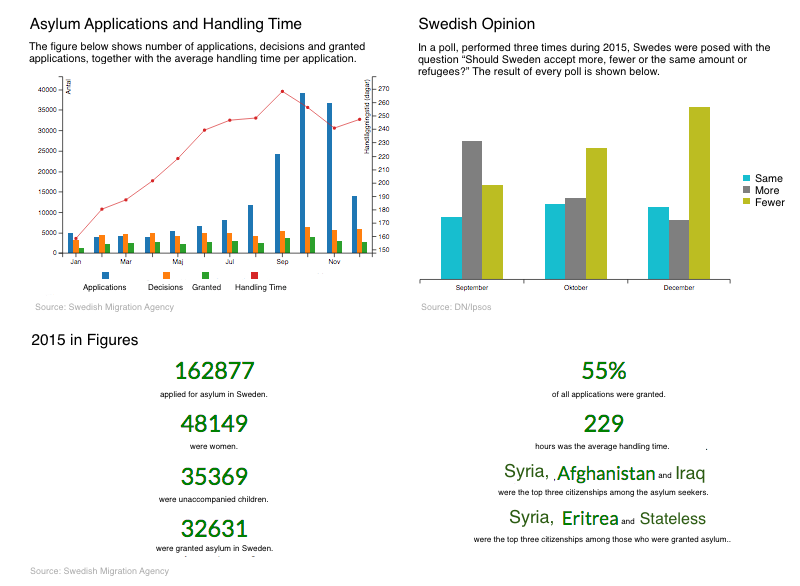
\includegraphics[width=\textwidth]{img/view2_en.png}
\caption{The asylum view. The visualization on the left shows a summary of applications, decisions, granted applications and average handling time during 2015. On the left there is a chart showing the Swedish opinion regarding refugees and at the bottom some key figures are presented in text. Note: the text has been translated to English in this thesis, however, the web app is in Swedish. For a short video showing the tool, follow this link: https://vimeo.com/187571807.}
\label{fig:view2}
\end{figure*}

\section{Method}
\label{sec:method}
In this section we will explain the methodology that we decided on, to research the question posed in Section \ref{sub:rq}. First, we can note that there are several ways of testing user interfaces. Choosing a methodology is not dependent only on the research question and what you want to test, but also on the interface itself, in particular where in the development phase you are. AsylKoll is in a very early stage of development, which needs to be taken into account when running the user-studies. If there are many bugs and the design is too rough, there is a risk that these obstacles disturb the users to such an extent that they are not able to properly test the interface. Thus, producing insufficient amount of data with such a quality that it is valuable to analyze. 

One way of getting around this problem of early stage testing, is presented by \citet{kinnaird2010focus}. A method used in the development of \emph{Connect 2 Congress} \cite{kinnaird2010connect}. The authors conducted their experiment by using focus groups, but instead of letting the users interact directly with the visualizations, two \emph{facilitators} participated in the study as well. The facilitators were familiar the the software and operated it for the users, in addition to recording the session and taking notes.

However, AsylKoll is built as a web interface and intended to be a window into Swedish immigration data, for non-experts. Thus, one key aspect is to analyze the behavior of first time users, who for some reason enter the website. Therefore, using a facilitator to guide the participants of the user-studies, might take away this effort to mimic the behavior of new users. Instead we have tried to develop and test the user interface, to such an extent that, it is simple and fast enough. Meaning that any imperfections in the software are so small that they will not interfere with the evaluations of the user-studies. To help understand how the users think when interacting with the software, we use a method called the \emph{Think Aloud Method}, which we describe in the next section \cite{someren1994think}.

\subsection{The Think Aloud Method}
\label{sub:think_aloud}
Solving a problem can be thought of as the the process of finding out the answer to a question without knowing the answer in advance. This is, in essence, what we are asking users to do when we want them to find their own stories, i.e. create reader-driven stories. With the help of a tool, in this study AsylKoll, we want the users to articulate stories of their own, without prior knowledge of what those stories might be, in order to make them learn and get a more fact-based world view. Therefore, for us to understand what users need to facilitate this learning process, we need to know what their \emph{thought processes} look like. Because given a task or a problem, people can end up with the exact same answer but the thought process of how they arrived at that answer can look very different. The Think Aloud Method is well suited for making it possible to evaluate these cognitive processes and the differences of them, between individuals.

As the name suggests, the method works such that the participants are asked to continuously think aloud and speak their mind, while using the software. The participants are asked to describe how they perceive the visualizations; how they go about understanding them; what is surprising about both the data and the visualizations; what they think is missing; what additional data they would like to compare the existing data with and so forth.

The data captured from the think aloud experiments is called \emph{verbal protocols}, which simply is some kind of record of what the participants are saying. This data can be captured in various ways, e.g. taking notes, audio or video recording. The verbal protocols are later coded according to a coding scheme, defined to help evaluate parameters of interest. The coding scheme used in this thesis is described in Section \ref{subsub:coding}.

\subsection{Experimental Setup}
\label{sub:exp}

\subsubsection{User-Studies}
\label{subsub:user_studies}
There are many ways of conducting a user-study with the Think Aloud Method. One common way is to evaluate single users, while they interact with the software. However, it can be difficult for people doing this type of experiment for the first time to be comfortable and speak their mind freely. For this reason we decided to conduct the study with groups instead and use a variant of the Think Aloud Method, called \emph{Dialog Observation}.

In Dialog Observation the participants solve tasks together. Tasks where they need to collaborate and communicate in order to solve them. This method was chosen since it is generally simpler for people that are not used to doing individual think aloud sessions. The discussions help the participants communicate in a more relaxed way, thus, providing more data for evaluation.

Two user-studies were performed. The first with four participants and the second with three. In both user-studies one administrator was also present, taking notes and recording the session on video. The administrator did not participate in the discussion, only reminding the participants to keep on talking if they went silent for too long. The video recordings were later used for analysis.

During both user-studies the participants were given the same two tasks:
\begin{enumerate}
\item Explore and familiarize yourself with the data and the visualizations
\item Construct four tweets that you find interesting and newsworthy
\end{enumerate}

The participants were not given the second task until the first one was finished. There were no strict time limits for any of the tasks and the first task was ended by the administrator, when the participants seemed to have explored the data sufficiently and the discussion naturally came to an end. Then they were given the second task, with the requirements that the tweets had to be fact-based and that every tweet had to include a screenshot from the tool, supporting the text in the tweet. All tweets can be found in appendix \ref{appen:tweets}.

\citet{someren1994think} lists two important conditions to consider when deciding on which tasks participants are asked to perform:
\begin{itemize}
\item Task should be at a level of difficulty that is appropriate for the subjects with respect to the cognitive process
\item The task should be representative with respect to the cognitive process involved
\end{itemize}

The cognitive process here can be understood as the process of constructing stories of your own, through data exploration. We would argue that the two tasks, presented earlier in this section, meets the conditions listed above. The first task is a prerequisite for understanding how a new user would perceive and interact with the tool, when presented with it for the first time. The second task is representative to the process of creating stories, since every tweet is a short story of its own. It is, however, hard to assess the correct level of difficulty. Nonetheless, writing a tweet is better than instead of e.g., a short news article, which would a possible option. Because a tweet is so short that it ought not to be an obstacle for participants who are not used to or comfortable with writing texts. At the same time, being limited to only 140 signs forces the participants to carefully construct the sentences, in order for them to be descriptive and newsworthy. Requiring the participants to always include a picture makes it easier to see how they use the tool and what they find interesting in the data.

Finally, given the fact that the data concerns a very polarized political topic in Sweden and that the participants were asked to agree on the tweets, they had to collaborate and discuss to complete the task. 

\subsubsection{Coding Scheme}
\label{subsub:coding}
To be able to evaluate the verbal protocols, i.e. the video recordings, they were \emph{segmented} and later \emph{classified} \cite{someren1994think}. The segments were delimited by either a natural end to the discussion, i.e. longer pause or a change of topic. Hence, a segment can be defined as a coherent discussion about one topic. 

Next, the segments were classified, according to the coding scheme shown in Table \ref{tab:scheme}. The segments were classified in two levels. A high-level, which classifies \emph{what} was being discussed (VIS, DA and ME), and a low-level, which classifies \emph{how} the discussed feature/subject affected the participants (RE, IN and ME). This is a simple coding scheme, focused on evaluating the parameters presented in the research question (see Section \ref{sub:rq}), and not intended to be exhaustive.

\begin{table}[!ht]
\tbl{Coding scheme used when analyzing the verbal protocols.}{
\begin{tabular}{p{0.5cm}p{1.5cm}p{5cm}}
\textbf{Code} & \textbf{Name} & \textbf{Description} \\
\hline
VIS & Visualizations & Discussion about the visualizations \\
DA & Data & Discussion about the data \\
ME & Meta & Everything that is not classified as DA, VIS, RE or IN \\
RE & Reader Engagement & Discussions/comments that say something about reader engagement \\
IN & Insights & Discussion/comments about how the participants gain insight/learn from the tool
\end{tabular}}
\label{tab:scheme}
\end{table}

\subsubsection{Survey}
\label{subsub:survey}
In order to capture whether the participants learned anything from the tool, how well it facilitated data exploration by non-exports and if they found the data interesting, the participants were asked to answer a short survey at the end of the session. The survey consisted of four Likert scale questions (scale 1-5). The questions in the survey were:
\begin{enumerate}
\item Did you learn something new about the asylum immigration in Sweden?
\item Did you find anything in the data surprising?
\item Was it difficult to understand the visualizations?
\item Was it difficult to interact with the tool?
\end{enumerate}
The result of the survey is shown in Section \ref{sub:results_survey}.

\section{Results}
\label{sec:results}
In this section we present the results of our two user-studies, including the surveys. The results are discussed in the next section, in Section \ref{sec:discussion}.

\subsection{User-Studies}
\label{sub:results_user_studies}
% TODO: Figure or high level discussion
% TODO: Table with important features that affect RE and IN

In Figure \ref{fig:segments} we present the statistics from the user-study. More specifically, we show the distribution of the high-level codes, derived during the analysis of the segments. The distribution of high-level codes are also shown in Table \ref{tab:high-level} and low-level codes in Table \ref{tab:low-level}. 

All tweets produced during user-study 1 and 2 can be found in appendix \ref{appen:tweets}.

\begin{figure}[!ht]
\centering
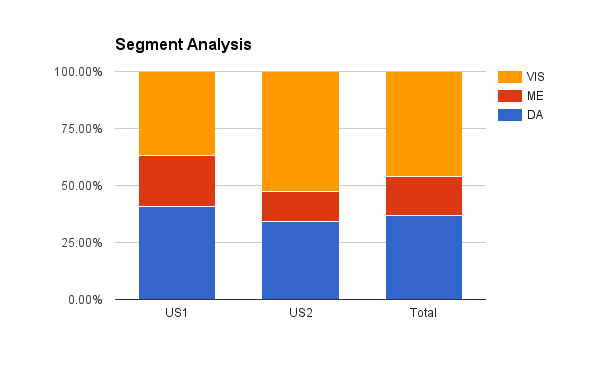
\includegraphics[width=8cm]{img/segments.png}
\caption{Distribution of high-level codes from both user-studies (VIS - discussion about the visualizations, DA - discussion about the data, ME - everything that is not classified as DA or VIS).}
\label{fig:segments}
\end{figure}

\begin{table}[!ht]
\tbl{High-level codes, in both user-studies.}{
\begin{tabular}{p{1cm}p{1cm}p{1cm}}
\textbf{Code} & \textbf{US1} & \textbf{US2} \\
\hline
VIS & 10 & 20 \\
DA & 11 & 13 \\
ME & 6 & 5
\end{tabular}}
\label{tab:high-level}
\end{table}

\begin{table}[!ht]
\tbl{Low-level codes, in both user-studies.}{
\begin{tabular}{p{1cm}p{1cm}p{1cm}}
\textbf{Code} & \textbf{US1} & \textbf{US2} \\
\hline
ME & 6 & 5 \\
RE & 4 & 5\\
IN & 17 & 28
\end{tabular}}
\label{tab:low-level}
\end{table}

\subsection{Survey}
\label{sub:results_survey}
The results of the survey that the participants were asked to complete at the end of the session, are shown in Figures \ref{fig:q1} - \ref{fig:q4} below.

\begin{figure}[!ht]
\centering
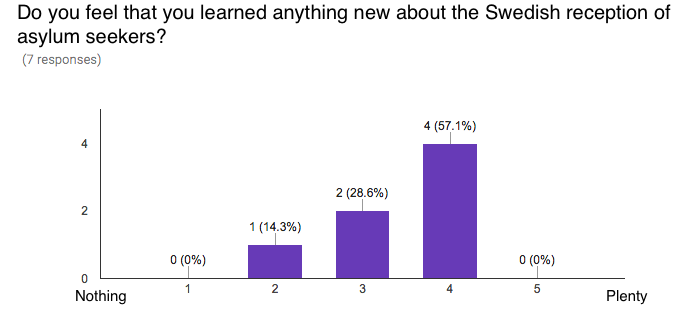
\includegraphics[width=8cm]{img/q1_en.png}
\caption{The results from question 'Do you feel that you learned anything new about the Swedish reception of asylum seekers?'. Scale 1-5, where 1 is 'plenty'.}
\label{fig:q1}
\end{figure}

\begin{figure}[!ht]
\centering
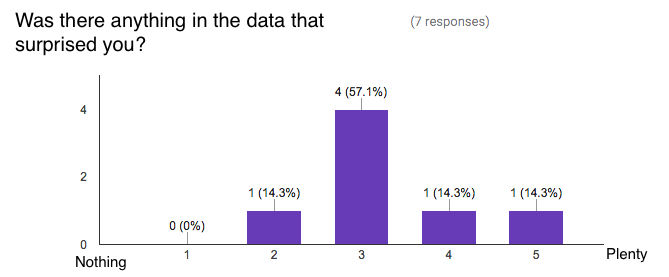
\includegraphics[width=8cm]{img/q2_en.png}
\caption{The results from question 'Was there anything in the data that surprised you?'. Scale 1-5, where 1 is 'nothing' and 5 is 'plenty'.}
\label{fig:q2}
\end{figure}

\begin{figure}[!ht]
\centering
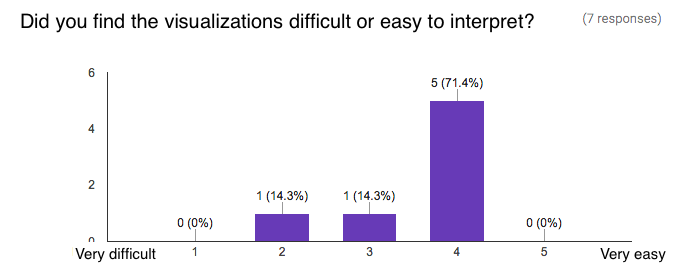
\includegraphics[width=8cm]{img/q3_en.png}
\caption{The results from question 'Did you find the visualizations difficult or easy to interpret?'. Scale 1-5, where 1 is 'very difficult' and 5 is 'very easy'}
\label{fig:q3}
\end{figure}

\begin{figure}[!ht]
\centering
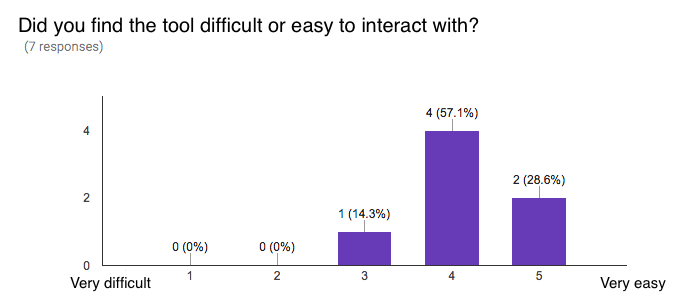
\includegraphics[width=8cm]{img/q4_en.png}
\caption{The results from question 'Did you find the tool difficult or easy to interact with?'. Scale 1-5, where 1 is 'very difficult' and 5 is 'very easy'.}
\label{fig:q4}
\end{figure}

\section{Discussion}
\label{sec:discussion}
% TODO: Add more stuff from related works?

In this section we will discuss and reflect on the outcomes of the analysis of the data that was gathered from the two user-studies and surveys. The general impression is indeed that AsylKoll already, at its current state, is able to help users articulate their own data-driven stories. During the user-studies the data and the visualizations spurred the participants into several different discussion about asylum immigration in Sweden. About cause and effect and how to utilize the data to create better integration. All in all, it was obvious that the topic was one of great interest. 

Breaking down the discussions into segments and coding these yielded the result shown in Figure \ref{fig:segments}. From that figure we see that even though the visualizations were discussed the most, there were almost as much discussions about the data itself. That is a positive result, since the data is key to a fact-based world view. The visualizations are only ways to facilitate the process of spreading that world view and the optimal result would be that all discussions were about the data. However, the result shown in Figure \ref{fig:segments} is especially good, given that the participants were in fact encourage to discuss the visualizations, to provide data about improvements of the tool. Nevertheless, the participants quickly got a grasp of how to use the tool and the data. Something that is supported by their answers to question 3 and 4 in the survey (see Figure \ref{fig:q3} and Figure \ref{fig:q4}).

Furthermore, an apparent finding, when analyzing the users' behavior, is the importance and the difficulty of using explanatory text together with the visualizations. A finding which partly confirms what has earlier been observed in \citet{borkin2016beyond,segel2010narrative}. In both focus groups, the importance of text was shown through the fact that reading the text was the first action for all participants. However, the users read the text quickly and not very carefully, which resulted in them missing several important instructions. Even though the explanatory text in the tool was only a few sentences in total. Hence, the text did little to help the participants figure out how to use the visualizations, contrary to what much of the previous research say. We see this as an apparent difficulty of using text.

Therefore, we would argue that one should \textbf{use text as little as possible} by trying to create the visualizations where very few text-based instructions are needed. Show instead the interactivity of a visualization by using various effects, e.g. change color or size on mouse-over, or use an introductory video that shows the user how the visualizations work. If text is needed, emphasize important instructions somehow, e.g. size, color or font style.

When looking at the stories produced during the two user-studies, i.e. the tweets (see appendix \ref{appen:tweets}), there are several interesting observations we can make. First, we note that the tweets from the two user-studies are similar, even though the studies were performed independent from each other. Figure \ref{fig:tweet1_3} and Figure \ref{fig:tweet2_3} show that \textbf{finding extremes} and \textbf{comparing} are important features when finding stories. Next, from Figure \ref{fig:tweet1_4} and Figure \ref{fig:tweet2_1}, we see that both groups found the data on the arrivals' country of origin interesting. In general, the participants seemed to be interested in finding stories \emph{about} those who came to Sweden during 2015. E.g. besides country of origin, the participants liked that age data was provided too. We interpret this as an interest to \textbf{humanize the data}. Indeed, if the data is in fact human data, as in AsylKoll, interest can be evoked by attaching human attributes to the abstract statistics and visualization.

There were also some indicators missing in AsylKoll. One thing, which was mentioned on different occasions by both groups, was the interest to correlate the data with media somehow. Since the topic of asylum immigration has been a hot topic in Sweden during the last year, media has written a lot about refugees and everything related to refugees, e.g. conflict zones. For this reason, it would have been good to include some kind of data on relevant news articles. Perhaps a window similar to what was included in Connect 2 Congress \cite{kinnaird2010connect}. Another indicator that both groups asked for and discussed was income. In fact, \textbf{income seems to be an indicator which attracts a lot of interest}.

A notable obstacle for having users derive reader-driven stories, related to media and the use of statistics in general, surfaced during the user-studies. Multiple participants tried to figure out what the author was trying to say with the data and the visualizations, despite that the tool was built to present the data as plain as possible, in order to avoid the presence of any author-driven stories. This source criticism is a sound approach to statistics, since there are many abusive ways of using it. However, if the goal is to let users find their own studies, this attitude can take precious focus from the data and instead change it to finding stories that are not there. In worse case, the user might refuse to see the data as facts. 

\subsection{Reader Engagement}
\label{sub:disc_re}
As has been mentioned earlier, in Section \ref{sub:reader_engagement}, in this thesis we wanted to see if we could increase reader engagement by focusing on the data, i.e. by using geographic-centric data relevant to the user. We would argue that this is indeed possible. The choropleth map in AsylKoll was the visualization that got the most attention. After reading text, which was the first action of all the participants, they immediately started to analyze the map. Discussing which county welcomed the most refugees and which who welcomed the least. The map also seemed to be easy for everyone to understand and extract information from. 

Once the participants figured out that it was possible to zoom in on a county by clicking the map they wanted to explore the extremes and the county where they lived. Using local data did increase reader engagement and it seems like it might be a good idea to use as local data as possible. AsylKoll presents data on municipality level but in both focus groups the users wanted to explore on an even more local level. Thus, \textbf{making the data as user-centric as possible}. 

There are also some conclusions which can be drawn regarding how to make users interact with the visualizations. In both focus groups the number of interactions were quite few in the beginning but as soon as they pass a certain threshold, the participants start clicking and exploring the visualizations much more. Therefore, it is important to ensure that the users are encouraged to interact with the visualizations as quickly as possible. E.g. if the users are presented with several different visualizations, it is advisable to let the users face simple, interactive visualizations at first. This will help the users if they are faced with a more complex visualization later, since they will be more willing to explore it.

A final observation was the positive correlation between visualizations with \textbf{details-on-demand} and how the participants engaged with the data and the visualizations, i.e. the reader engagement.

\subsection{Learning}
\label{sub:disc_le}
By looking at Figure \ref{fig:q1} and Figure \ref{fig:q2} we can conclude that the participants felt they did learn new things about asylum immigration in Sweden, by using AsylKoll. When analyzing the video recordings there are some features that are recurring for both groups, regarding what helps them gain insights and learn from the data and the visualizations.

One frequent request for example, mentioned earlier in this section, was the ability to \textbf{make comparisons} both within and between geographical-levels. E.g. comparing counties, comparing a municipality with a county, comparing a municipality with the country as a whole. Moreover, the participants were interested in \textbf{finding the extremes}, minimum and maximum, for all geographical levels. In addition, the provided \textbf{details-on-demand} had a positive impact on how the participants drew insights and learned from the tool. In addition, there was a need expressed to always present absolute numbers together with relative numbers. Absolute numbers alone evoke interest but \textbf{absolute numbers in conjunction with relative numbers provide understanding}.

\section{Conclusions and Future Work}
\label{sec:conclusion} 
In this thesis we set out to explore the domains of reader-driven stories by performing user-studies on a very basic tool, AsylKoll, which shows immigration data in Sweden. From this initial and limited study we have seen that even a simple and minimalistic visualization tool, such as AsylKoll, has the potential to spark fruitful discussions and raise questions, which fuel a need for further exploration. Essential requirements for having users successfully discover their own data-driven stories.

From our user-studies we have been able to gain both general insights about visualizations that support the articulation of reader-driven stories. However, we chose to focus on exploring how to create visualizations that maximize reader engagement and ensure learning. We found that reader engagement can be increased by doing the following:
\begin{itemize}
\item Center the data around the users
\item Encourage users to start interacting with the visualizations as soon as possible to maximize the number of interactions
\item Use a lot of transitions, mouse-over effects and details-on-demand
\end{itemize}
Similarly, we find that it is possible to boost learning by providing features which enable users to easily:
\begin{itemize}
\item Make comparisons
\item Find extreme values
\item Extract a lot of additional data through details-on-demand
\item Explore absolute numbers in conjunction with relative numbers
\end{itemize}

However, this study is merely a first glance into the vast research space of reader-driven stories. Looking ahead, gathering quantitative data, instead of qualitative as in this study, will be essential. E.g. by publishing the tool on a web page with a lot of visitors and analyzing how users interact with the tool. The data generated would valuable for several reasons. It would i) mimic first user behavior better than those group discussions used in this thesis; ii) possible impact that the administrator had on the participants would be controlled; and iii) the data would come from a much wider sample of user types. Furthermore, a more advance coding scheme, than the one used in this thesis, could be used by including more categories and, thus, providing more detailed insights about users' behavior. 

In conclusion, in a world with an ever increasing supply of data and a continuous abuse of statistics and facts, we firmly believe that reader-driven stories have an important role to play in the quest of spreading a fact-based world view.

% FUTURE WORK

% Already a lot of stories about this in Sweden - push to a web site and use updated data and gather individual data
% My presence might affect creative process - push to a web site and gather individual data
% Being a group might not perfectly mimic the behavior of a new user - push to a web site and gather individual data
% Include some experts too, see how they usually go about using visualizations to find stories and have that as a comparison for how non-expert go about performing the task - push to a web site and gather individual data
% Users, they were all from collage - push to a web site and gather individual data

% To this: Store states of what people investigate, make available to general public, analyze what stories people explore
% to remedy above

% Simple analysis made (only three categories on every levels) - make more advanced coding and analysis, many things to discover except RE and LE

% How to overcome the problem of ensuring participants nothing is ''meant'' by the data?

% Specifically, we believe that this will help the user find short stories and micro learning

% Confident that reader-driven stories have an important role to play in the quest of spreading a fact-based world view. 

%%%%%%%%%% ACKNOWLEDGEMENTS %%%%%%%%%%
%\newpage

%\vspace{0.5cm}
\begin{acks}
We are grateful to the following people for resources, discussions and
suggestions.

Mario; for support, coaching and positive energy, without which this thesis would have been a far greater struggle.

Ola; for the opportunity to work at such a great foundation. Angie, Fernanda, Gabriela, Jasper, Mattias, Max and Åsa; for a warm welcome, valuable insights and many laughs. 

Elisabeth, Eric, Erik, Filip, Mariam, Mathias and Viktor; for lending the project your amazing brains and thus, providing the means needed to finish this thesis.
\end{acks}

%%%%%%%%%% BIBLIOGRAPHY %%%%%%%%%%

\bibliographystyle{ACM-Reference-Format-Journals}
\bibliography{sources}

%%%%%%%%%% APPENDIX %%%%%%%%%%

\newpage
\appendix

\section{Tweets}
\label{appen:tweets}
This section includes all the tweets produced during both user-studies.

\begin{figure}[!hb]
\centering
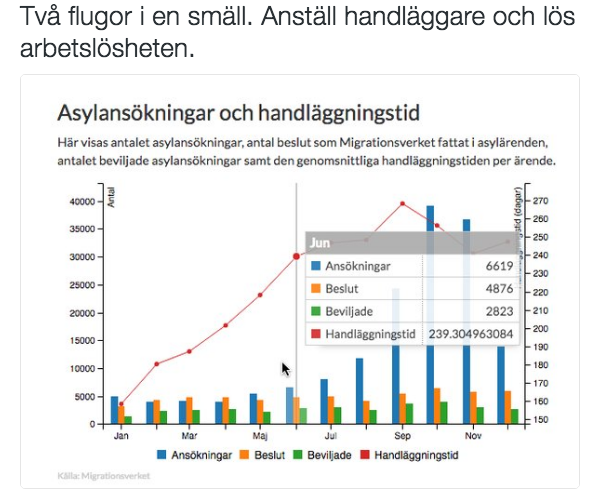
\includegraphics[width=8cm]{img/tweet1_1.png}
\caption{Tweet from user-study 1.}
\label{fig:tweet1_1}
\end{figure}

\begin{figure}[!hb]
\centering
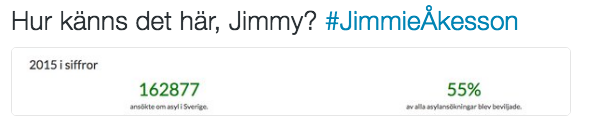
\includegraphics[width=8cm]{img/tweet1_2.png}
\caption{Tweet from user-study 1.}
\label{fig:tweet1_2}
\end{figure}

\begin{figure}
\centering
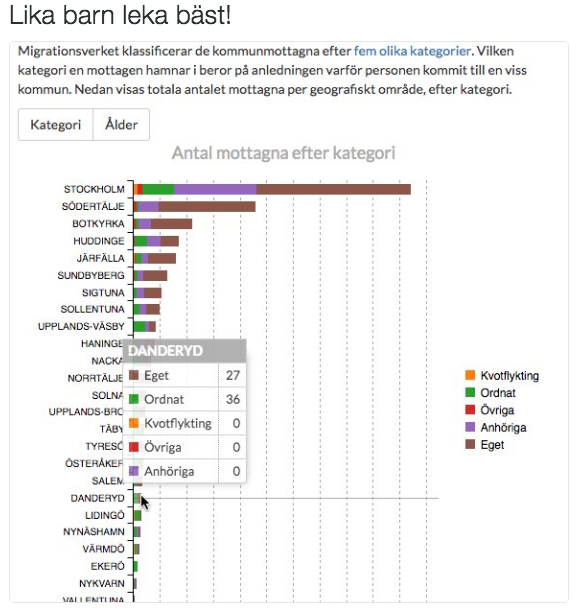
\includegraphics[width=8cm]{img/tweet1_3.png}
\caption{Tweet from user-study 1.}
\label{fig:tweet1_3}
\end{figure}

\begin{figure}
\centering
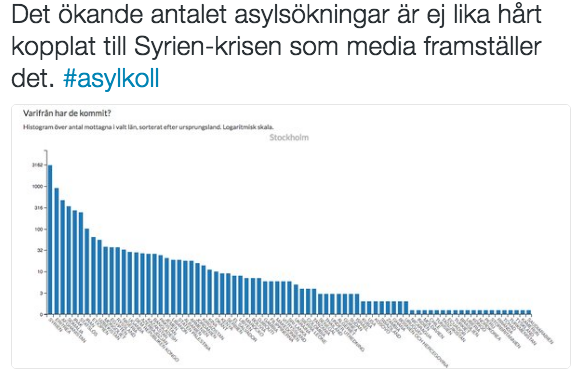
\includegraphics[width=8cm]{img/tweet1_4.png}
\caption{Tweet from user-study 1.}
\label{fig:tweet1_4}
\end{figure}

\begin{figure}
\centering
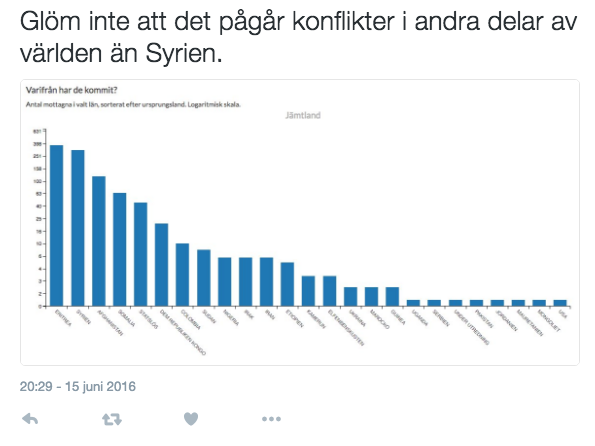
\includegraphics[width=8cm]{img/tweet2_1.png}
\caption{Tweet from user-study 2.}
\label{fig:tweet2_1}
\end{figure}

\begin{figure}
\centering
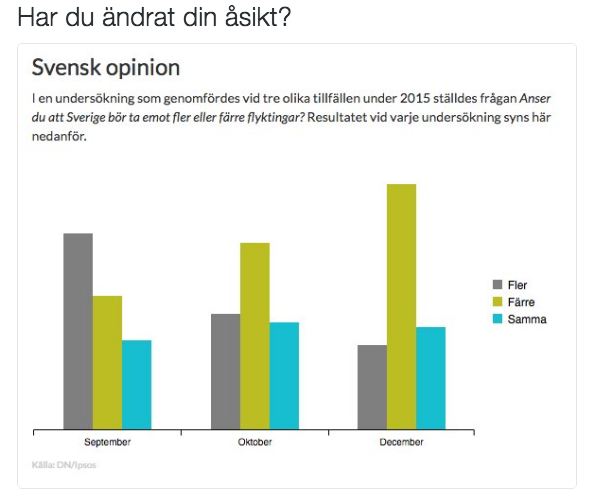
\includegraphics[width=8cm]{img/tweet2_2.png}
\caption{Tweet from user-study 2.}
\label{fig:tweet2_2}
\end{figure}

\begin{figure}
\centering
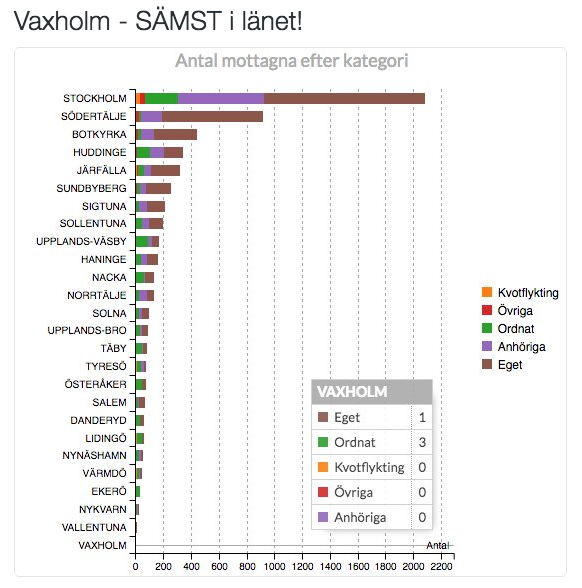
\includegraphics[width=8cm]{img/tweet2_3.png}
\caption{Tweet from user-study 2.}
\label{fig:tweet2_3}
\end{figure}

\begin{figure}
\centering
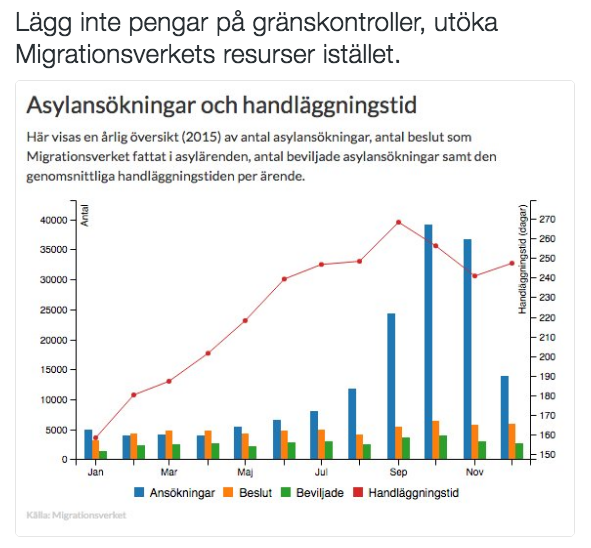
\includegraphics[width=8cm]{img/tweet2_4.png}
\caption{Tweet from user-study 2.}
\label{fig:tweet2_4}
\end{figure}



%%%%%%%%%%%%%%%%%%%%%%%%%%%%%%%%%%%%%%%%%%%%%%%%%%%%%%%%%%%%%%%%%%%%%%%%%%%%%%%%%%%%%%%%%%%%%%%%%%%%%%%%%%%%%%%%%%%%%


% COMMENTS AND SHIT
\begin{comment}
RELATED WORKS


Visualization pipeline ?
Taxonomy to follow
Vitruvius triangle

'At a minimum, stories concern temporal sequences - situations and events unfolding in time.' \cite{herman2011basic}

As \citet{tufte1990envinf} writes ''clutter and confusion are failures of design, not attributes of information''.

\cite{hullman2013contextifier} automatically produce custom stories to data in order to increase understanding?

A good definition for narrative visualization in \cite{scopemore} 

Important research to create a taxonomy 


which encompasses several different subfields, e.g. computer science, psychology, design. However, to generalize it is, as is hinted in the name, a marriage of information visualization and storytelling. In this section we will describe relevant research in both these two subfields before merging them and ending the section with current research in narrative visualization.


\section{Information Visualization}
Information visualization can be understood as 'the use of computer-supported interactive visual representations of abstract data to amplify cognition.' \cite{card1999readings}.

Beautiful qoute from \cite{tufte1990envinf} 'to envision information - and what bright and splendid visions can result - is to work at the intersection of image, word, number, art'.

Narrative information visualization is a young and emerging field within information visualization but nevertheless interesting research has already been conducted. In order to align the research presented in this paper with existing research in information visualization the taxonomy used in this paper stems from several well-known sources \cite{amar2004,fffffffffman1996eyes,amar2005low,chi2000taxonomy}.

Tips on how to design information visualization and what needs that should be met have been researched \cite{amar2004,amar2005low}

\section{Storytelling}

Something from \cite{herman2011basic} and perhaps \cite{blundell1988art}.

\section{Narrative Visualization}

Some kind of definition in \cite{hullman2011visualization}

First to notice the use of adding stories to visualization were \cite{gershon2001storytelling}.


Author-driven versus reader-driven, and design space \cite{segel2010narrative}


There is reasearch that refutes that adding adding introductory stories to exploratory visualization increases user-engagement \cite{boy2015can}. 

Research on which narrative visualizations that have the desried outcome, i.e. conveying a story, on the readers is still quite unexplored. Therea are no clear models for narrative visualization. However, some research give directions on how to create a story that people understand and remember \cite{borkin2016beyond}.

The curse of dimensionality, i.e. showing high-dimensional data is difficult \cite{bertini2011quality}.

Discuss and compare \cite{chi2000taxonomy,card1999readings,north2009visualization}, i.e. the visualization pipleline.
\end{comment}

\end{document}
% End of v2-acmtog-sample.tex (March 2012) - Gerry Murray, ACM
